\chapter{Konzept}
\label{chapter_Konzept}

Im folgenden Kapitel wird auf die Erstellung des Konzeptes eingegangen.

\section{Teststand}
\label{section_Teststand}

Das Gesamtsystem setzt sich aus drei Untersystemen zusammen:

\begin{itemize}

\item Mess-Client
\begin{itemize}
\item Übernimmt die lokale Ansteuerung der \acp{DUT}
\item Nimmt Messdaten auf und stellt sie zur Verfügung
\end{itemize}

\item Mess-Server
\begin{itemize}
\item Verwaltet angeschlossene Mess-Clients
\item Speichert alle Messdaten
\item Bildet das Bindeglied zwischen Mess-Client und dem PC-Client
\end{itemize}

\item PC-Client
\begin{itemize}
\item Parametriert die Mess-Clients
\item Wertet Messdaten aus und stellt sie leserlich da
\end{itemize}

\end{itemize}


\begin{figure}[H]
\begin{center}
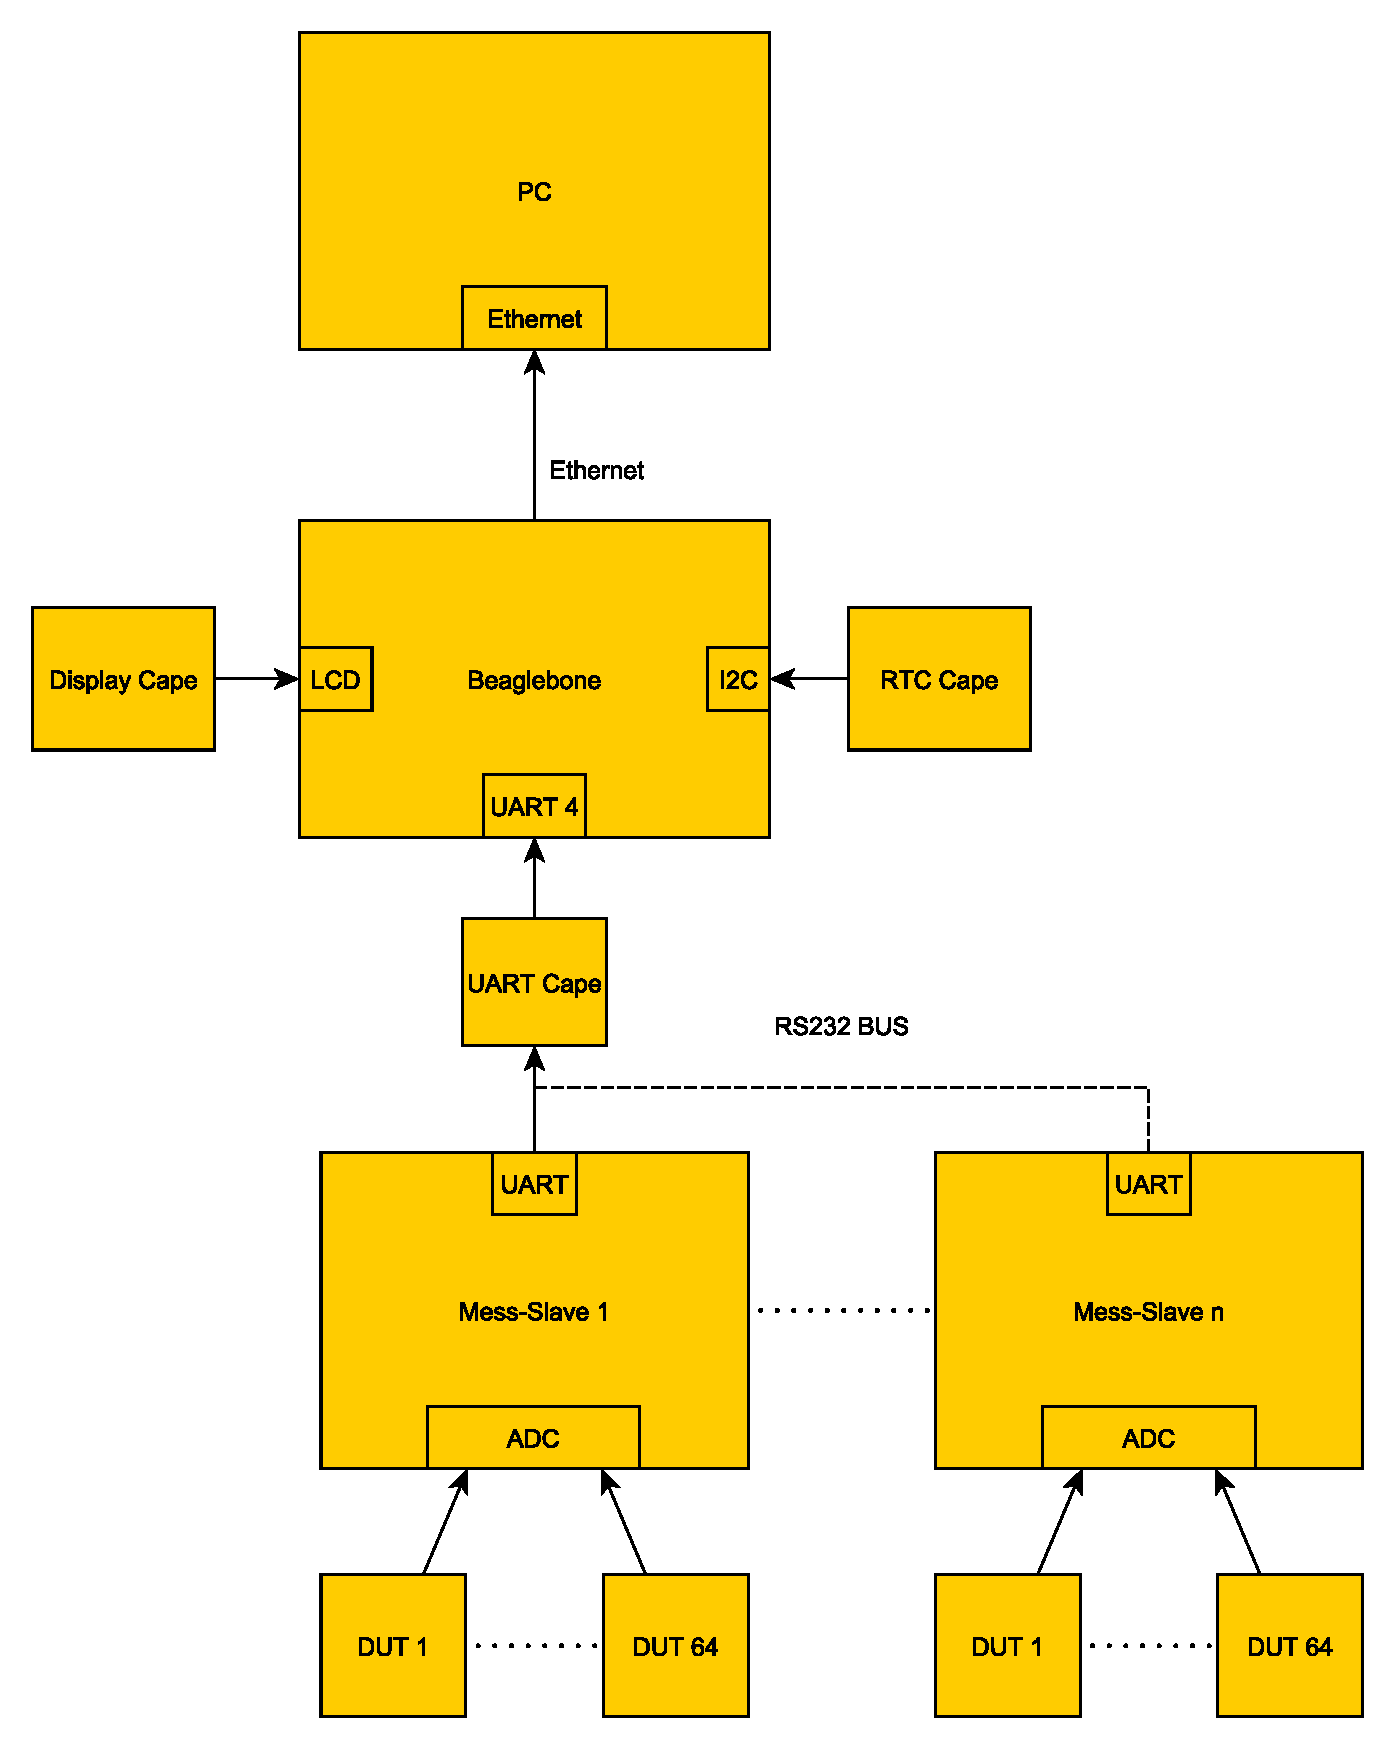
\includegraphics[width=\textwidth]{img/general/BlockPlan.pdf}
\caption{Gesamt System}
\label{Gesamt_System}
\end{center}
\end{figure}


\subsection{Mess-Client}
\label{section_Mess-Client}

Das Herzstück des Mess-Clients bildet ein STM8  8-Bit Mikrocontroller der Firma STMicroelectronics.
Auf jedem Mess-Client sind 64 \acp{DUT} befestigt. In zyklischen Abständen werden die Messdaten der Prüfobjekte aufgenommen und über eine RS232-Schnittstelle zur Verfügung gestellt (siehe Abbildung \ref{MessSlaveBlockPlan}.\\
Dieses System war zum großen Teil bereits gegeben, so dass lediglich die Übertragung der RS232 Schnittstelle geregelt werden musste. Dazu wurde ein Protokoll für die Kommunikation entworfen (sieht Abschnitt \ref{section_RS232_Protokoll}).
 

%\begin{figure}[h]
%\begin{center}
%\includegraphics[width=\textwidth]{}
%\caption{Mess-Client Blockschaltplan}
%\label{MessSlaveBlockPlan}
%\end{center}
%\end{figure}

\newpage
\subsection{Mess-Server}
\label{section_Mess-Server}

Als Mess-Server wird ein BeagleBone Black von Texas Instruments eingesetzt. Dabei handelt es sich um einen kostengünstigen Einplatinencomputer der mit einem AM335x 1GHz ARM® Cortex-A8 Prozessor arbeitet. Des Weiteren verfügt er über 512MB DDR3 RAM und 4GB 8-bit eMMC internen Flash Speicher.


\begin{figure}[H]
\begin{center}
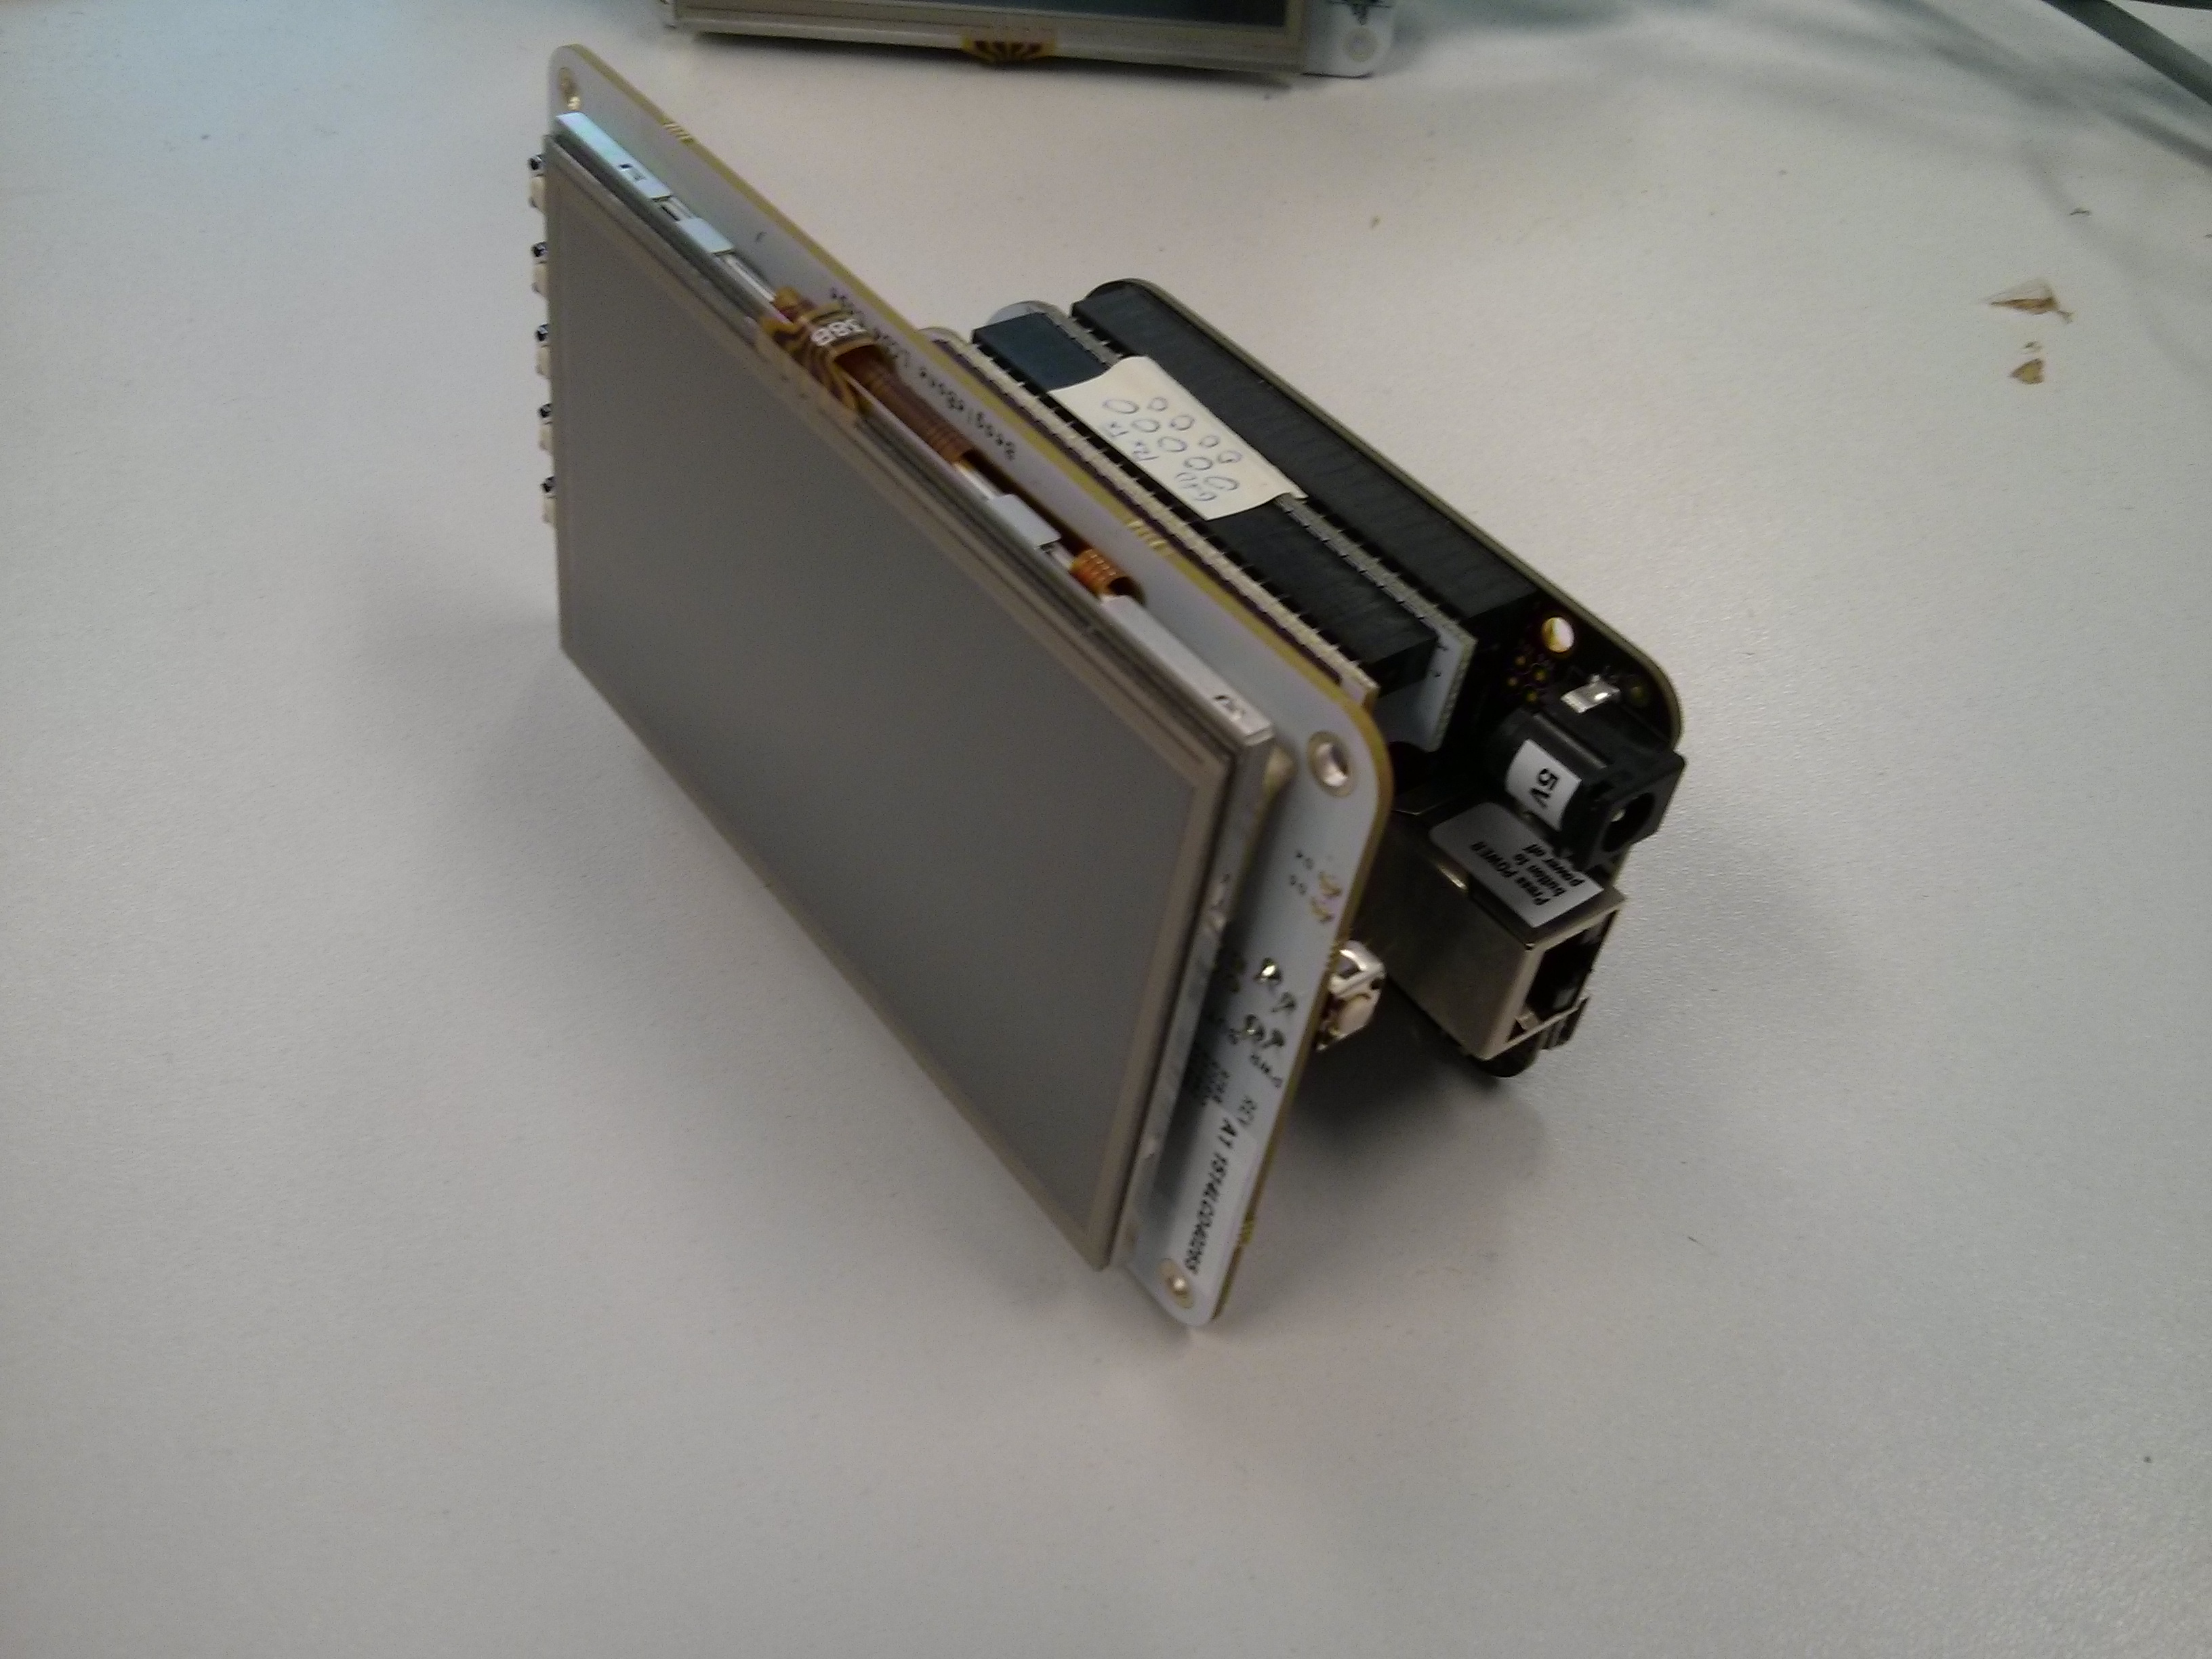
\includegraphics[width=\textwidth]{img/general/BeagleBoneBlack.jpg}
\caption{BeagleBone Black}
\label{figure_Beagleboneblack}
\end{center}
\end{figure}

Trotz der Kompaktheit des BeagleBone Black, bietet er ein ausreichendes Maß an Performance. Auf ihm kommt ein Debian-GNU/Linux Betriebssystem zum Einsatz. Damit ist es möglich die umfangreichen Debian-Funktionen wie die Paketverwaltung zu nutzen. Es bietet auch den Vorteil, dass eine große Ähnlichkeit zu PC-Distributionen wie Ubuntu besteht und somit einfacher nutzbar ist(vgl. \cite{schroeder2009embedded}).\\
Außerdem sind Linux Mechanismen einfach nutzbar. So kann das \ac{UART} Interface beispielsweise wie eine normale Datei beschrieben und gelesen werden.

\subsubsection{Aufbau}


\begin{figure}[H]
\begin{center}
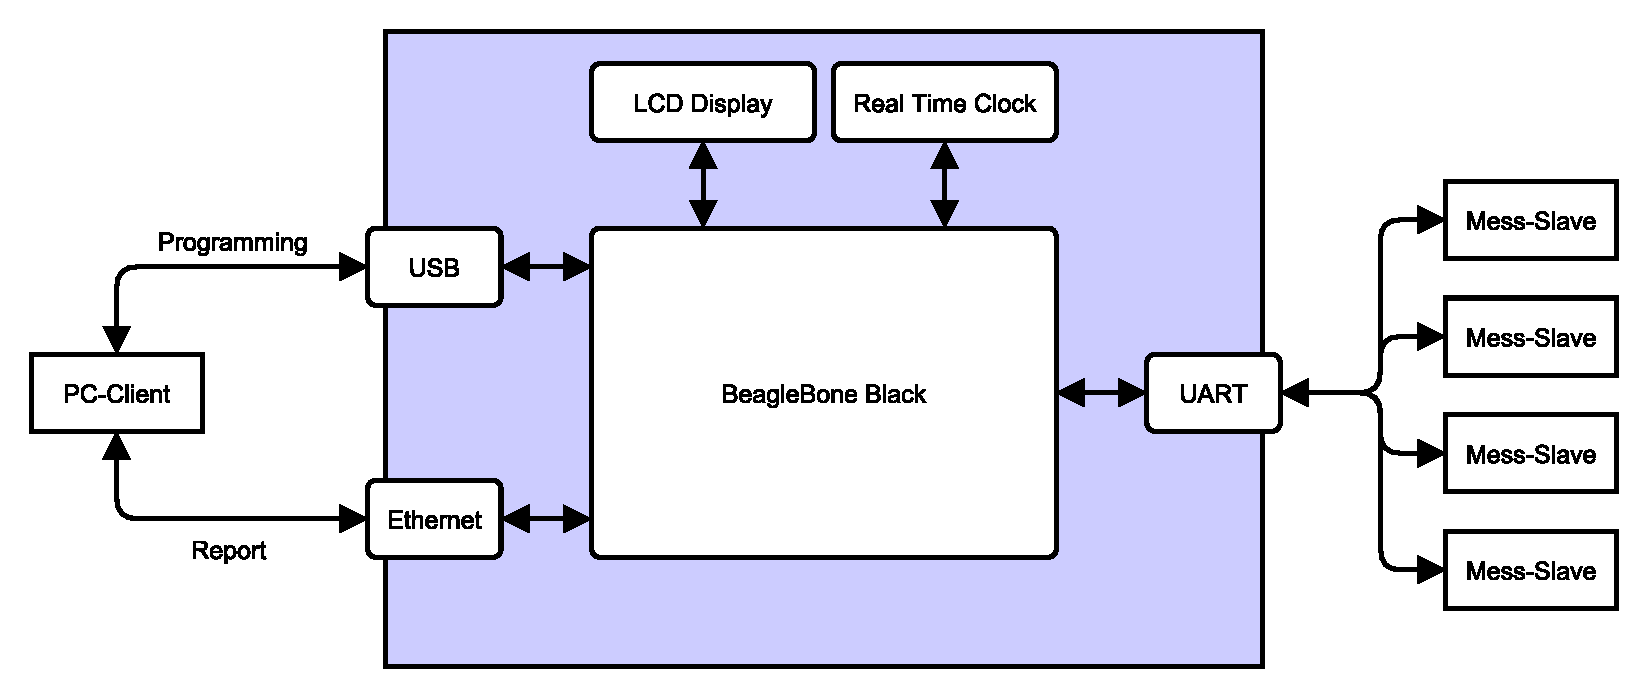
\includegraphics[width=\textwidth]{img/general/UebersichtMaster.pdf}
\caption{Aufbau BeagleBone Black}
\label{figure_AufbauBleagleBone}
\end{center}
\end{figure}

Das BeagleBone Black bildet das Herzstück des Systems.



\newpage
\subsection{PC-Client}
\label{section_Verwaltung}
asdasad

\newpage
\section{RS232 Protokoll}
\label{section_RS232_Protokoll}
Das Protokoll für die Kommunikation über die RS232 Schnittstelle dient zum Austausch von Informationen innerhalb des Systems zwischen den Akteuren. \\

Folgende Kriterien sollen dabei erfüllt werden:
\begin{itemize}
\item Adressierung individueller Kommunikationspartner
\item Senden verschiedener Befehle
\item Variable Größe der Daten
\item Sicherstellung der Validität der Übertragung
\item Erweiterbar
\end{itemize}



Um eine hohe Zuverlässigkeit gewährleisten zu können, wird eine geringe Bautrate von 2400 verwendet. Da nur geringe Datenmengen in großen Abständen auftreten, vermindert dass die Anfälligkeit der Übertragung gegenüber äußeren Einflüssen ohne dabei die Performance merkbar zu beeinflussen.\\
Des Weiteren wird ein Paritätsbit für eine Paritätsprüfung eingesetzt. Dieses Bit gibt an, ob die Anzahl der Einsen des Datenblocks gerade oder ungerade ist. Der Wert verwendeten Even-Paritätsbit ist 1, wenn die Summe der Einsen gerade ist und 0 wenn sie ungerade ist. Dadurch können grobe Fehler bei der Übertragung ausgemacht und korrigiert werden.
\newpage
\subsection{Aufbau}
\begin{table}[H]
\begin{center}
\begin{tabularx}{\textwidth}{|c|c|c|c|X|X|}\hline
 1. Byte & 2. Byte & 3. Byte & 4. Byte & 5. Byte und folgend & Letztes Byte\\ \hline
  Adresse \& R/W & Länge & Befehl & Unterbefehl & Nutzdaten & Checksumme\\ \hline
\end{tabularx}
\caption{Übertragungsrahmen}
\label{table_Frame}
\end{center}
\end{table}

Ein Rahmen des Protokolls besteht aus 4 Steuerbytes, 1 Checksummenbyte und maximal 30 Bytes an Nutzdaten. Durch diesen Aufbau können die Anforderungen erfüllt werden. Im folgenden Abschnitt wird auf die Zusammensetzung und die Funktion der einzelnen Bytes eingegangen.\\




\textbf{1. Byte: Adresse \& Read/Write}

\begin{table}[H]
\begin{center}
\begin{tabularx}{\textwidth}{|X|X|X|X|X|X|X|X|}\hline
 7. Bit & 6. Bit & 5. Bit & 4. Bit & 3. Bit & 2. Bit & 1. Bit & 0. Bit\\ \hline
 R/W & Addr6 & Addr5 & Addr4 & Addr3 & Addr2 & Addr1 & Addr0\\ \hline
\end{tabularx}
\caption{1. Byte: Adresse \& Read/Write}
\label{table_1Byte}
\end{center}
\end{table}

Das erste Byte des Übertragungsrahmens setzt sich aus 7 Adressbits und einem Lese-/Schreibbit zusammen. Die ersten 7 Bit (Addr0 - Addr6) bilden die Adresse des anzusteuernden Empfänger. Daraus ergibt sich ein Adressraum von möglichen 128 Adressen, wobei Adresse 0 für neue Mess-Clients zur einmaligen Anmeldung im System reserviert ist (siehe Abschnitt \ref{section_messclientverwaltung}).\\
Das höchste Bit ist das Lese-/Schreibbit. Mithilfe dieses Bits wird unterschieden, ob ein Befehl als Lese- oder Schreibzugriff interpretiert werden soll.\\

\begin{table}[H]
\begin{center}
\begin{tabular}{|l|l|}\hline
 R/W Bit & Beschreibung \\ \hline
 0 & Die Sender möchte lesen \\ \hline
 1 & Die Sender möchte schreiben \\ \hline
\end{tabular}
\caption{Read/Write}
\label{table_RW}
\end{center}
\end{table}

Ein Lesezugriff stellen dabei Anfragen dar. Dass heißt, dass keine Nutzdaten übertragen werden und eine Antwort des Empfängers mit den angeforderten Daten erwartet wird. Bei einem Schreibzugriff hingegen, werden immer Nutzdaten übertragen.\\

\newpage

\textbf{2. Byte: Rahmenlänge}

\begin{table}[H]
\begin{center}
\begin{tabularx}{\textwidth}{|X|X|X|X|X|X|X|X|}\hline
 7. Bit & 6. Bit & 5. Bit & 4. Bit & 3. Bit & 2. Bit & 1. Bit & 0. Bit\\ \hline
 Len7 & Len6 & Len5 & Len4 & Len3 & Len2 & Len1 & Len0\\ \hline
\end{tabularx}
\caption{2. Byte: Rahmenlänge}
\label{table_2Byte}
\end{center}
\end{table}

Das zweite Byte gibt die Länge des gesamten Rahmens inklusive Steuerbytes, Nutzdaten und Checksumme an. Die minimale Rahmenlänge beträgt 5 Byte. Dabei handelt es sich um eine Übertragung ohne Nutzdaten und es werden lediglich die 4 Steuerbytes und das Byte für die Checksumme übertragen. Dies geschieht beispielsweise bei einer Leseanfrage.\\
Die maximale Rahmenlänge beträgt 35 Byte. Hierbei werden zusätzlich zu den 4 Steuerbytes und dem Byte für die Checksumme auch die maximale Nutzlast von 30 Byte übertragen. Dieser Fall kann beispielsweise bei Schreibzugriffen auftreten.\\
Anhand der Länge kann eine erste Prüfung der Validität eines Rahmens durchgeführt werden. Sollte die Zahl der empfangenen Bytes sich von der Rahmenlänge unterscheiden, kann von einem ungültigen Rahmen ausgegangen werden.\\



\textbf{3. Byte: Befehl}

\begin{table}[H]
\begin{center}
\begin{tabularx}{\textwidth}{|X|X|X|X|X|X|X|X|}\hline
 7. Bit & 6. Bit & 5. Bit & 4. Bit & 3. Bit & 2. Bit & 1. Bit & 0. Bit\\ \hline
 Cmd7 & Cmd6 & Cmd5 & Cmd4 & Cmd3 & Cmd2 & Cmd1 & Cmd0\\ \hline
\end{tabularx}
\caption{3. Byte: Befehl}
\label{table_3Byte}
\end{center}
\end{table}

Das dritte Byte repräsentiert den Befehl. Dieser gibt an, welche Aktion ausgeführt oder welcher Parameter angesprochen wird. Da insgesamt ein Byte für den Befehl zur Verfügung steht, sind bis zu 256 unterschiedliche Befehle möglich.\\

\newpage

\textbf{4. Byte: Unterbefehl}

\begin{table}[H]
\begin{center}
\begin{tabularx}{\textwidth}{|X|X|X|X|X|X|X|X|}\hline
 7. Bit & 6. Bit & 5. Bit & 4. Bit & 3. Bit & 2. Bit & 1. Bit & 0. Bit\\ \hline
 Scmd7 & Scmd6 & Scmd5 & Scmd4 & Scmd3 & Scmd2 & Scmd1 & Scmd0\\ \hline
\end{tabularx}
\caption{4. Byte: Unterbefehl}
\label{table_4Byte}
\end{center}
\end{table}

Das vierte Byte ist der Unterbefehl. Damit ist es möglich einen Befehl genauer zu spezifizieren. So kann beispielsweise der Befehl zum Auslesen eines \ac{ADC} Wertes durch den Unterbefehl genau auf einen von 64 \acp{ADC} präzisiert werden. Im späteren Verlauf wird in Abschnitt \ref{section_BefehleUnterbefehle} näher auf die vorhandenen Befehle und Unterbefehle eingegangen.\\



\textbf{5. Byte und folgend: Nutzdaten}

\begin{table}[H]
\begin{center}
\begin{tabularx}{\textwidth}{|X|X|X|X|X|X|X|X|}\hline
 7. Bit & 6. Bit & 5. Bit & 4. Bit & 3. Bit & 2. Bit & 1. Bit & 0. Bit\\ \hline
 Data7 & Data6 & Data5 & Data4 & Data3 & Data2 & Data1 & Data0\\ \hline
\end{tabularx}
\caption{5. Byte und folgend: Nutzdaten}
\label{table_5Byte}
\end{center}
\end{table}

Das fünfte Byte und die darauf folgenden, tragen die Nutzdaten des Rahmens. Die Größe der Nutzdaten ist variable und lässt dich auf der Rahmenlänge ableiten. Bei zwei Byte Daten wird immer das höhere Byte zuerst übertragen.\\


\newpage

\textbf{Letztes Byte: Checksumme}

\begin{table}[H]
\begin{center}
\begin{tabularx}{\textwidth}{|X|X|X|X|X|X|X|X|}\hline
 7. Bit & 6. Bit & 5. Bit & 4. Bit & 3. Bit & 2. Bit & 1. Bit & 0. Bit\\ \hline
 CKS7 & CKS6 & CKS5 & CKS4 & CKS3 & CKS2 & CKS1 & CKS0\\ \hline
\end{tabularx}
\caption{Letztes Byte: Checksumme}
\label{table_LastByte}
\end{center}
\end{table}

Das letzte Byte ist immer die Checksumme um sicherzustellen, dass alle Daten komplett und fehlerfrei übertragen wurden.\\
Der Sender bildet dabei die Checksumme mittels einer XOR Verknüpfung aller Bytes eines Übertragungsrahmens. Beim Empfänger werden alle Bytes inklusive Checksumme erneut mit XOR Verknüpft, wobei ohne Fehler immer 0 das Ergebnis sein muss.\\


\textbf{Beispiel}

Sender:
 
Es wird angenommen das folgender Rahmen übertragen wird.
\begin{center}
\begin{tabular}{|c|c|c|c|}\hline
  Adresse & Länge & Befehl & Unterbefehl \\ \hline
  1 & 5 & 9 & 0 \\ \hline
\end{tabular}
\end{center}
Aus dem Rahmen wird dann mittels XOR die Checksumme gebildet.

\begin{center}
{\Large$1 \oplus 4 \oplus 9 \oplus 0 = 13$}\\
\end{center}

Anschließend wird die Checksumme als letztes Byte an den Rahmen an gehangen.
\begin{center}
\begin{tabular}{|c|c|c|c|c|}\hline
  Adresse & Länge & Befehl & Unterbefehl & Checksumme \\ \hline
  1 & 5 & 9 & 0 & 13 \\ \hline
\end{tabular}
\end{center}

Empfänger:

Sobald der Empfänger den rahmen erhält, verknüpft er alle Bytes erneut mittels XOR um die Gültigkeit zu prüfen.

\begin{center}
{\Large $1 \oplus 4 \oplus 9 \oplus 0 \oplus 13 = 0$}\\
\end{center}

Das Ergebnis 0 repräsentiert einen gültigen Rahmen und die Checksummenprüfung war erfolgreich.


\subsection{Befehle und Unterbefehle}
\label{section_BefehleUnterbefehle}
Für die Funktion des Systems sind verschiedene Befehle notwendig. Sie dienen zu Kommunikation zwischen den Akteuren.
Eine Übersicht über die implementierten Befehle der RS232 Schnittstelle findet sich in Tabelle \ref{table_RS232Commands}.\\

\begin{table}[H]
\begin{center}
\begin{tabularx}{\textwidth}{|X|c|X|c|}\hline 
 Befehl & Code & Unterbefehl & Datenbytes \\ \hline \hline
 ADC-Value & 0x00 & MUX-Kanal (0..63) & 2  \\ \hline
 Number Of Pulses & 0x04 & - & 1  \\ \hline
 Pulsewidth and -period & 0x05 & Pulsnummer (1..20) & 4  \\ \hline
 Perform Pulseupdate & 0x06 & - & 0   \\ \hline
 DAC-Value & 0x07 & - & 2 \\ \hline
 Temperature & 0x08 & - & 1  \\ \hline
 LTT Name & 0x09 & - & 1..30  \\ \hline
 Rs232-Address & 0x0A & - & 1 \\ \hline
 Measurement Intervall & 0x0C & Intervallnummer (0..2) & 4 \\ \hline
\end{tabularx}
\caption{RS232 Befehlsliste}
\label{table_RS232Commands}
\end{center}
\end{table}

\textbf{ADC-Value}\\
Der Befehl liest den Messwert eines Sensors des Mess-Clients. Mit dem Unterbefehl muss einer der 64 Sensoren spezifiziert werden. Die Datenmenge beträgt 2 Byte.\ 

\textbf{Number Of Pulses}\\
Dieser Befehl liest oder schreibt die Anzahl der Impulse im Pulsmuster des Mess-Clients. Die maximale Anzahl ist 20.\ 

\textbf{Pulsewidth and -period}\\
Ändert ein Pulsbreiten-/Pulsperiodenpaar. Der Unterbefehl bestimmt die Position im Pulsmuster.\ 

\textbf{DAC-Value}\\
Ließt oder schreibt den Wert für die Vorverstärkung zur Ansteuerung der Prüfobjekte.\ 

\textbf{Temperatur}\\
Der Befehl ließt den Wert des Temperatursensors.\ 

\textbf{LTT Name}\\
Ließt oder schreibt des Namen des Kommunikationspartners.\ 

\textbf{RS232-Adresse}\\
Ließt oder schreibt die Adresse für die Rs232 Kommunikation des Kommunikationspartners.\ 

\textbf{Measurement Intervall}\\
Ließt oder schreibt die Konfiguration der Messintervalle. Der Unterbefehl gibt dabei den Zeitraum (1 bis 3) an.\ 




\newpage
\section{Datenbank}
\label{section_EntwurfDatenbank}

Aus den Anforderungen ergibt sich folgendes \ac{ERM} (siehe Abbildung \ref{ERM}). \\

\begin{figure}[H]
\begin{center}
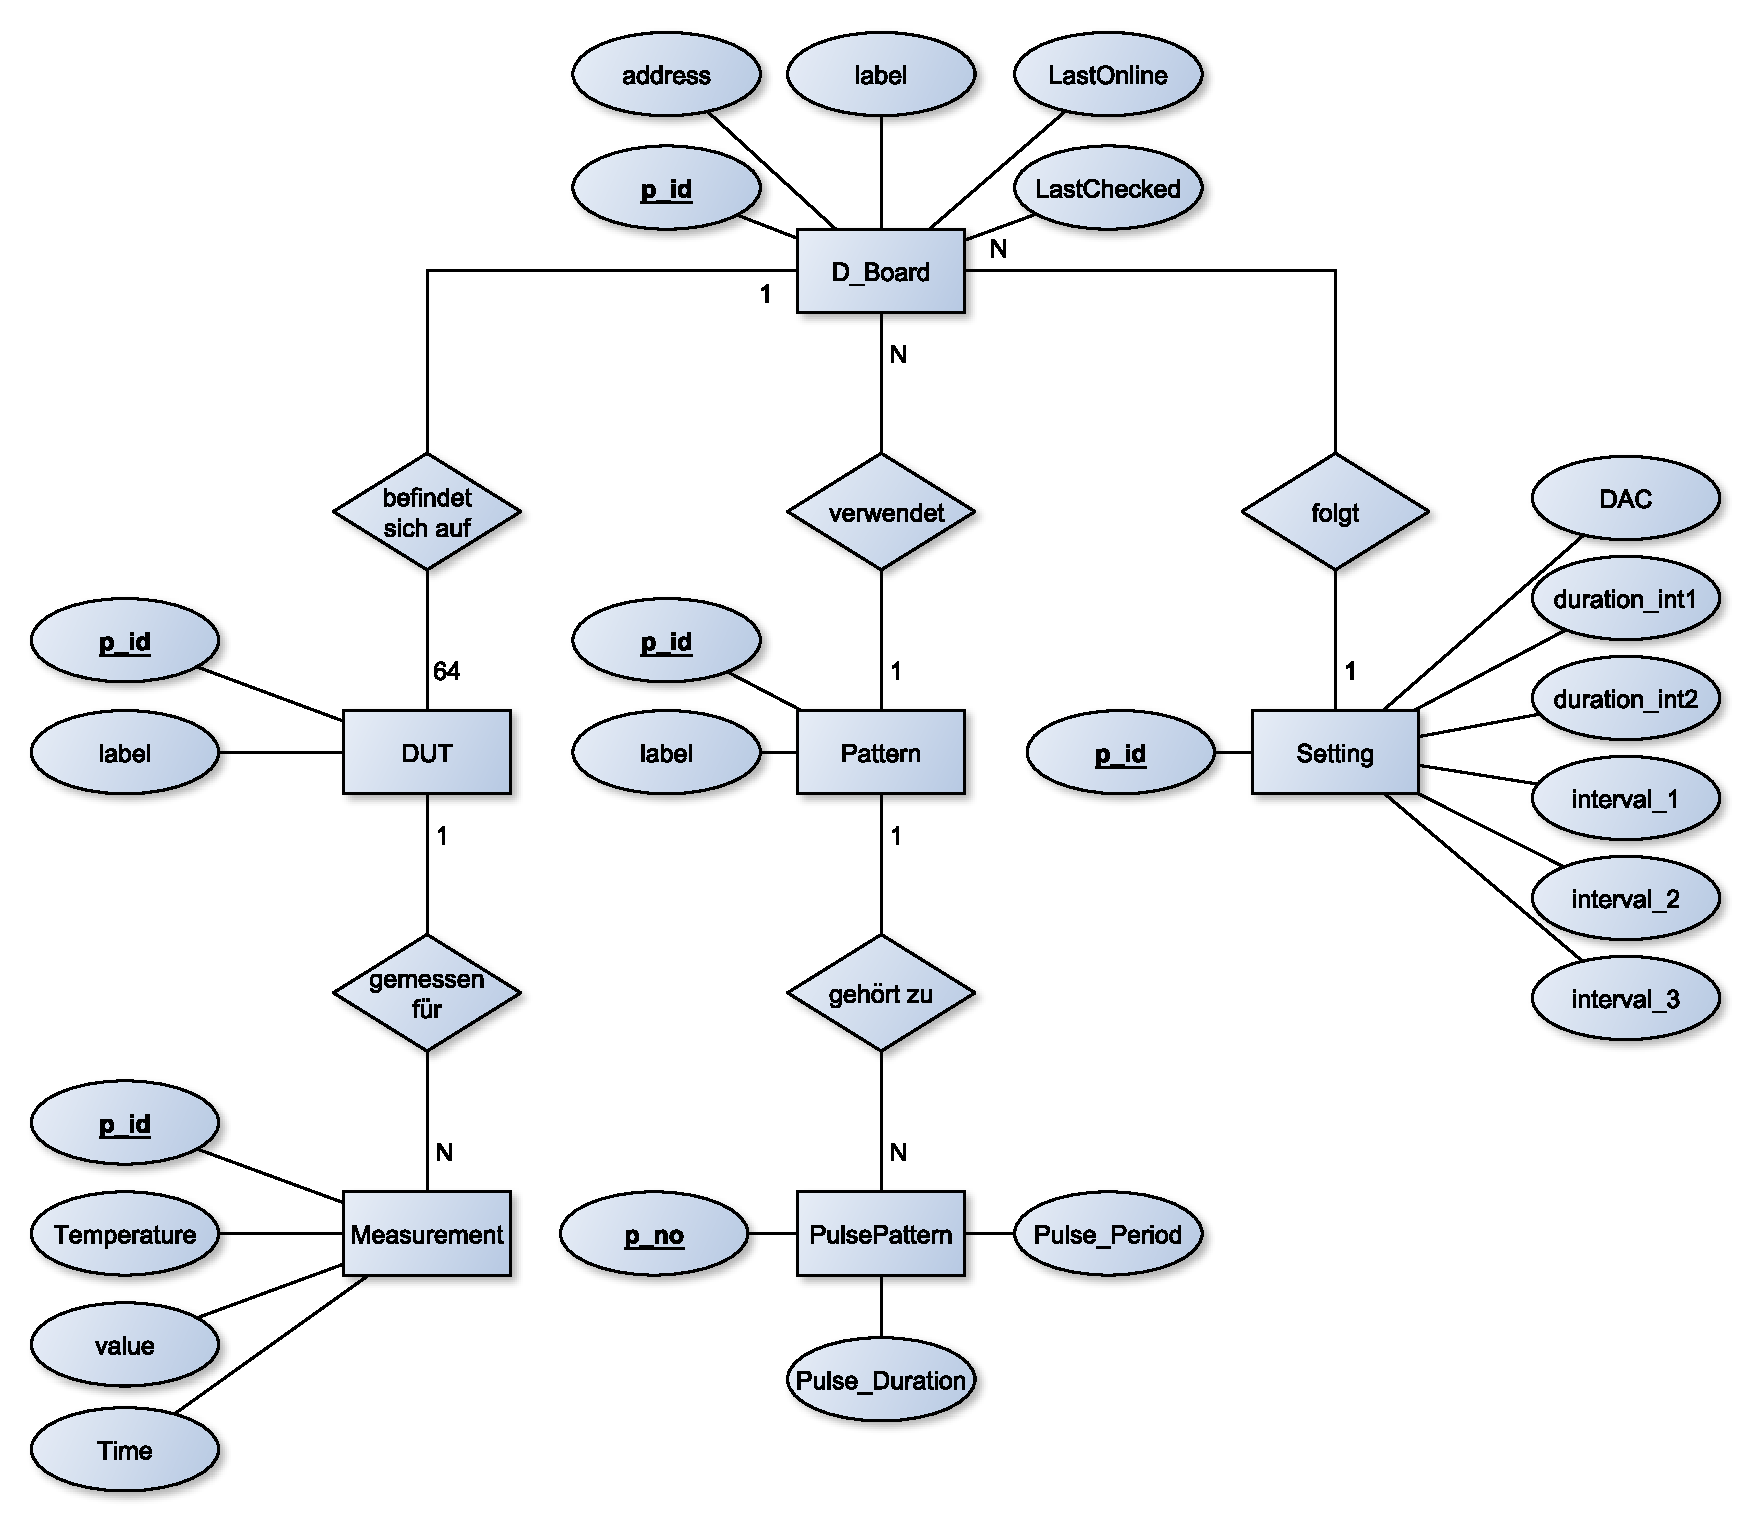
\includegraphics[width=\textwidth]{img/general/ER_Diagramm.pdf}
\caption{Entity Relationship Modell}
\label{ERM}
\end{center}
\end{figure}


Die Datenbank muss folgende Daten für die Parameter der Mess-Clients aufnehmen:\\

\begin{table}[H]
\begin{center}
\begin{tabular}{|l|l|}\hline
Parameter & Beschreibung \\ \hline
DAC & Vorverstärkung\\ 
duration\_int1 & Dauer der Zeit die Werte im 1.Interval aufgenommen werden in Tagen\\ 
duration\_int2 & Dauer der Zeit die Werte im 2.Interval aufgenommen werden in Tagen\\ 
interval\_1 & Abstand zwischen den Messungen im 1. Interval in Minuten\\ 
interval\_2 & Abstand zwischen den Messungen im 2. Interval in Minuten\\ 
interval\_3 & Abstand zwischen den Messungen nach dem 2. Interval in Minuten\\ \hline
\end{tabular}
\caption{Tabelle Setting}
\label{table_TabelleSetting}
\end{center}
\end{table}




